 \documentclass[10pt,a4paper]{article}
\usepackage[utf8x]{inputenc}
\usepackage{amsmath}
\usepackage{mathtools}
\usepackage{framed}
\usepackage{amsfonts}
\usepackage{hyperref}
\usepackage{float}
\usepackage{amssymb}
\setlength{\parindent}{0pt}
\usepackage{graphicx}
\usepackage{todonotes}
\usepackage{fullpage}
\usepackage{tikz}
\usetikzlibrary{calc,arrows}
\makeatletter
\pgfdeclareshape{circuit}{
  \savedanchor\northeast{
    \pgfmathsetlength\pgf@x{\pgfshapeminwidth}
    \pgfmathsetlength\pgf@y{\pgfshapeminheight}
    \pgf@x=0.5\pgf@x
    \pgf@y=0.5\pgf@y}
  \savedanchor\southwest{
    \pgfmathsetlength\pgf@x{\pgfshapeminwidth}
    \pgfmathsetlength\pgf@y{\pgfshapeminheight}
    \pgf@x=-0.5\pgf@x
    \pgf@y=-0.45\pgf@y}
  \inheritanchorborder[from=rectangle]
  \anchor{center}{\pgfpointorigin}
  \anchor{north}{\northeast \pgf@x=0pt}
  \anchor{east}{\northeast \pgf@y=0pt}
  \anchor{south}{\southwest \pgf@x=0pt}
  \anchor{west}{\southwest \pgf@y=0pt}
  \anchor{north east}{\northeast}
  \anchor{north west}{\northeast \pgf@x=-\pgf@x}
  \anchor{south west}{\southwest}
  \anchor{south east}{\southwest \pgf@x=-\pgf@x}
  \anchor{text}{
    \pgfpointorigin
    \advance\pgf@x by -.5\wd\pgfnodeparttextbox
    \advance\pgf@y by -0.1875\ht\pgfnodeparttextbox
    \advance\pgf@y by +.5\dp\pgfnodeparttextbox}
\anchor{ina}{
  \pgf@process{\northeast}
  \pgf@x=-1\pgf@x
  \pgf@y=0.5\pgf@y}
\anchor{outa}{
  \pgf@process{\northeast}
  \pgf@y=0.5\pgf@y}
\anchor{outb}{
  \pgf@process{\northeast}
  \pgf@y=0.09999999999999998\pgf@y}
\anchor{outc}{
  \pgf@process{\northeast}
  \pgf@y=-0.3\pgf@y}
\anchor{inb}{
  \pgf@process{\northeast}
  \pgf@x=-1\pgf@x
  \pgf@y=0.09999999999999998\pgf@y}
\anchor{outd}{
  \pgf@process{\northeast}
  \pgf@y=-0.7000000000000001\pgf@y}
\backgroundpath{
  \pgfpathrectanglecorners{\southwest}{\northeast}
  \begingroup
    \tikzset{labels}
    \tikz@textfont
  \endgroup}}
\tikzset{add font/.code={\expandafter\def\expandafter\tikz@textfont\expandafter{\tikz@textfont#1}}}
\tikzset{labels/.style={font=\sffamily\scriptsize}}
\tikzset{every circuit node/.style={draw,minimum width=2cm,minimum height=2.5cm,very thick,inner sep=1mm,outer sep=0pt,cap=round,add font=\sffamily\bfseries}}
\makeatother
\DeclarePairedDelimiter\ceil{\lceil}{\rceil}
\DeclarePairedDelimiter\floor{\lfloor}{\rfloor}
\newcount\colveccount
\newcommand*\colvec[1]{
        \global\colveccount#1
        \begin{pmatrix}
        \colvecnext
}
\def\colvecnext#1{
        #1
        \global\advance\colveccount-1
        \ifnum\colveccount>0
                \\
                \expandafter\colvecnext
        \else
                \end{pmatrix}
        \fi
}
\begin{document}
\section{ADC}
\subsection{Purpose of the ADC}
An ADC converter is needed for this project to convert the analog voltages which the photo diode create into an digital value which the digital logic need to determine the color of the block.   
The ADC component being used for this process will be the MCP3008, which is an 10 bit ADC converter.  
\subsection{MCP3008}
The MCP3008 is an ADC component, it is capable of converting an analog value from the ranging from 2.7 - 5.5 into an 10 bit value. It is rated to have an conversion rate of 200 ksps at an $V_{dd} = 5V$


\todo[inline]{\textbf{-- Billede af komponentn\\
}}
The chip has 16 pins, at which the pins to the left consist of 8 seperate input ports for analog voltages, and the right side consist of $V_dd, V_ref, AGND,CLK, CS, Dout, Din$.  The FPGA interfaces the with ADC using the pins CLK, CS, DOUT, DIN. 
The ADC uses an SPI-based interface to communicate with the FPGA. \\


The CLK consist of the clock frequency at which data will be sent to the ADC and read from the ADC. According to the datasheet is the max frequency for the comunication 3.57 mHz, which the FPGA provides it with at that port. The datasheet states that the min. clock rate has to be 10Khz as this will affect the linearity performance of the ADC,  and especially as different temperatures. \\


Din is the input port which the FPGA send the init bits to. 
ADC is only going to read an analog value from CHO, and convert into a digital value, hence the init bits the ADC should be provided with is "11000".  The first '1' bitt bit ,  The next '1' bit bit determines whether the system should perform a single ended or differential conversion. Single ended conversion converts the input from one port, and differential conversion converts the difference between two ports. '1' declares the conversion as an single ended conversion. The last 3 bits "000" determines the port at which it has to read from, in this case being from CH0.\\
  

Dout is the output port which the FPGA reads the converted analog value as an 10 bit digital binary number. When a conversion has been performed,  the first bit the which will be read from the Dout port will be the a null bit, and afterwards will each bit of the 10 bit be outputted from MSB to LSB. \\


CS is chip select. It is used to initiate communication between ADC and FPGA, when it is pulled low, when it is pulled high, it will end the conversion and put the ADC in a standby mode.  It must be pulled high between each new conversions. 
 

\todo[inline]{\textbf{-- diagram viser timing tingen -- \\
}}
\subsection{Implementation of communication}

The communication between MPC3008 and the FPGA is implemented as an entity named ADC. ADC consist of an state machine with 4 states. 
Idle, init, convert, transmit. \\
 
 


\begin{figure}[htb]
\centering
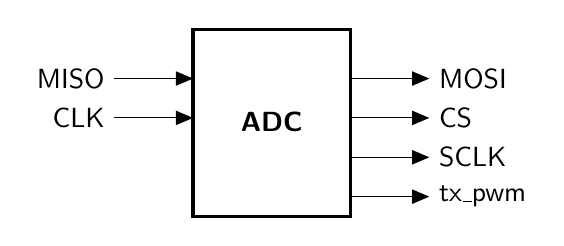
\begin{tikzpicture}[font=\sffamily,>=triangle 45]
  \node [shape=circuit] (item) at (0,0) {ADC};
  \draw [<-] (item.ina) node [anchor=west,labels] {} -- +(-1,0) node [anchor=east] {MISO};
  \draw [->] (item.outa) node [anchor=east,labels] {} -- +(1,0) node [anchor=west] {MOSI};
  \draw [->] (item.outb) node [anchor=east,labels] {} -- +(1,0) node [anchor=west] {CS};
  \draw [->] (item.outc) node [anchor=east,labels] {} -- +(1,0) node [anchor=west] {SCLK};
  \draw [<-] (item.inb) node [anchor=west,labels] {} -- +(-1,0) node [anchor=east] {CLK};
  \draw [->] (item.outd) node [anchor=east,labels] {} -- +(1,0) node [anchor=west] {tx\_pwm};
\end{tikzpicture}
\caption{Entity of ADC}
\end{figure}
 
The Idle states set the ADC into an standby mode, by setting the the CS high, and make it ready to convert a new Analog value.  The state machine will be on this state for one 1 clock event. \\

The init states sets up the component for conversion, by sending the init bits , bitwise from the MOSI port to the Din port of the MCP3008. 

\subsection{MCP3008 errors}
\subsection{Tests}

\section{Servo motor}
The purpose of the servo motor is control the "flipper", which separates the blocks. \\


A servo motor consist of an DC motor, potentiometer and a control circuit.  As the motoro rotates, the resistance of the potentiometer changes,  so that the control circuit can precisely movement and the direction.   When the motor shaft is at the desired position the power supplied to the motor will be used stop the motor, such that it doesn't move away from the desired position. \\

The desired position is sent through the sense wire, (often the white wire). The position  itself is defined as PWM signal where the duty cycle defines the position\\
 

-- Billede af PWM of duty cycle --  \\

The servo motor used in this project only turn from $0^{\circ}$ to $180^{\circ}$

To rotate the motor to the position 
\subsection{Interaction with Servo motor}
The control of the servo motor, is done using the FPGA with the entity named pwm. 

\begin{figure}[htb]
\centering
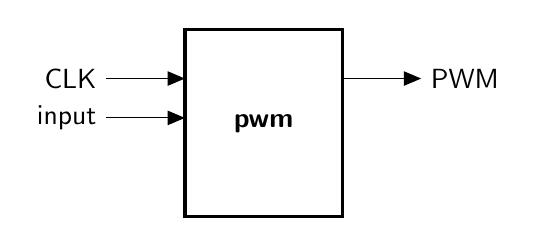
\begin{tikzpicture}[font=\sffamily,>=triangle 45]
  \node [shape=circuit] (item) at (0,0) {pwm};
  \draw [<-] (item.ina) node [anchor=west,labels] {} -- +(-1,0) node [anchor=east] {CLK};
  \draw [->] (item.outa) node [anchor=east,labels] {} -- +(1,0) node [anchor=west] {PWM};
  \draw [<-] (item.inb) node [anchor=west,labels] {} -- +(-1,0) node [anchor=east] {input};
\end{tikzpicture}
\caption{Entity of pwm}
\end{figure}

\section{LED - driver}
\subsection{Purpose of the LED - driver}
\subsection{Implementation}

\section{Control logic}
\subsection{Purpose of the Control logic}
\subsection{Implementation}

\section{Top module}

\end{document}